\documentclass[titlepage]{article}
\usepackage[utf8]{inputenc}
\usepackage[czech]{babel}
\usepackage{amsmath}
\usepackage{graphicx}
\usepackage{a4wide}
\usepackage[table]{xcolor}

\include{pygments}

\begin{document}
\begin{titlepage}
\begin{center}
	\mbox{} \\[3cm]
	\huge{1. semestrální práce z předmětu KIV/ÚPA} \\[2.5cm]
	\Large{Tomáš Maršálek, A10B0632P} \\
	\large{marsalet@students.zcu.cz} \\[1cm]
	\normalsize{\today}
\end{center}
\thispagestyle{empty}
\end{titlepage}



\section{Zadání}
\large{\textbf{Zadání semestrální práce - A10B0632P}}
\begin{itemize}
\item Navrhněte automat, který pracuje podle zobrazeného schématu.
\item Zvolte kódování stavů a vstupů (černá šipka představuje impuls I1,
		červená šipka představuje impuls I2). Pokud nepřichází žádný impuls, automat
setrvává v aktuálním stavu.
\item Zamyslete se, zda použijete synchronní nebo asynchronní klopné
obvody, a vhodně zvolte jejich typ (JK nebo D).
\item Vytvořte tabulku přechodů a výstupů se zakódovanými stavy, vstupy a
výstupy.
\item Sestavte Karnaughovy mapy budících a výstupních funkcí a provďte
minimalizaci. Tyto funkce zapište výrazem.
\item Nakreslete schéma zapojení obvodu.
\item Nezapomeňte na nulový vstup. Nulový vstup znamená, že nepřichází do
obvodu žádný vstupní signál (tj. na všechny vodiče vstupu přijde 0 - nebo 1,
		pokud si to tak zvolíte). Vzhledem k tomu, že máte ještě navíc další dva druhy
vstupních impulsů (I1, I2), nestačí vám jeden vodič pro vstup.
\end{itemize}

Výstupy obvodu jsou:

\begin{center}
\begin{tabular}{|c|c|c|c|c|c|}
\hline
{\bf A} & {\bf B} & {\bf C} & {\bf D} & {\bf E} & {\bf F} \\
\hline
x & y & z & z & y & x \\
\hline
\end{tabular}
\end{center}

\begin{figure}[ht!]
\centering
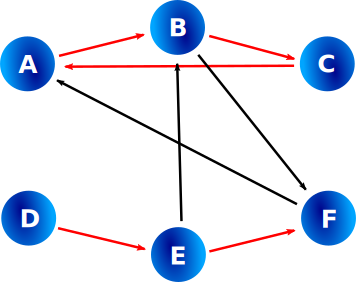
\includegraphics[width=10cm]{graf.pdf}
\end{figure}
\clearpage

\section{Kódování}
\subsection{Stavy}
\begin{center}
\begin{tabular}{|l|l|l|l|}
\hline
& {\bf $s_1$} & {\bf $s_2$} & {\bf $s_3$}\\
\hline
A & 0 & 0 & 0 \\
B & 0 & 0 & 1 \\
C & 0 & 1 & 0 \\
D & 0 & 1 & 1 \\
E & 1 & 0 & 0 \\
F & 1 & 0 & 1 \\
\hline
\end{tabular}
\end{center}

\subsection{Vstupy}
\begin{center}
\begin{tabular}{|l|l|l|}
\hline
& {\bf $x_1$} & {\bf $x_2$} \\
\hline
Nic & 0 & 0 \\
Červená & 0 & 1 \\
Černá & 1 & 0 \\
\hline
\end{tabular}
\end{center}

\subsection{Výstupy}
\begin{center}
\begin{tabular}{|l|l|l|}
\hline
& {\bf $y_1$} & {\bf $y_2$} \\
\hline
x & 0 & 0 \\
y & 0 & 1 \\
z & 1 & 0 \\
\hline
\end{tabular}
\end{center}


\begin{center}
\rowcolors{2}{gray!25}{white}
\begin{tabular}{|l|l|l|l|l|l|l|l|l|l|l|l|l|l|l|l|}
\hline
{\bf $x_1$} & {\bf $x_2$} & {\bf $s_1'$} & {\bf $s_2'$} & {\bf $s_3'$} & {\bf
$s_1$} & {\bf $s_2$} & {\bf $s_3$} & {\bf $y_1$} & {\bf $y_2$} & {\bf $j_1$} & {\bf $k_1$} & {\bf $j_2$} & {\bf $k_2$} & {\bf $j_3$} & {\bf $k_3$}\\
\hline
0 & 0 & 0 & 0 & 0 & 0 & 0 & 0 & 0 & 0 & 0 & - & 0 & - & 0 & - \\
\hline
0 & 0 & 0 & 0 & 1 & 0 & 0 & 1 & 0 & 1 & 0 & - & 0 & - & - & 0 \\
\hline
0 & 0 & 0 & 1 & 0 & 0 & 1 & 0 & 1 & 0 & 0 & - & - & 0 & 0 & - \\
\hline
0 & 0 & 0 & 1 & 1 & 0 & 1 & 1 & 1 & 0 & 0 & - & - & 0 & - & 0 \\
\hline
0 & 0 & 1 & 0 & 0 & 1 & 0 & 0 & 0 & 1 & - & 0 & 0 & - & 0 & - \\
\hline
0 & 0 & 1 & 0 & 1 & 1 & 0 & 1 & 0 & 0 & - & 0 & 0 & - & - & 0 \\
\hline
0 & 0 & 1 & 1 & 0 & - & - & - & - & - & - & - & - & - & - & - \\
\hline
0 & 0 & 1 & 1 & 1 & - & - & - & - & - & - & - & - & - & - & - \\
\hline
0 & 1 & 0 & 0 & 0 & 0 & 0 & 1 & 0 & 0 & 0 & - & 0 & - & 1 & - \\
\hline
0 & 1 & 0 & 0 & 1 & 0 & 1 & 0 & 0 & 1 & 0 & - & 1 & - & - & 1 \\
\hline
0 & 1 & 0 & 1 & 0 & 0 & 0 & 0 & 1 & 0 & 0 & - & - & 1 & 0 & - \\
\hline
0 & 1 & 0 & 1 & 1 & 1 & 0 & 0 & 1 & 0 & 1 & - & - & 1 & - & 1 \\
\hline
0 & 1 & 1 & 0 & 0 & 1 & 0 & 1 & 0 & 1 & - & 0 & 0 & - & 1 & - \\
\hline
0 & 1 & 1 & 0 & 1 & 1 & 0 & 1 & 0 & 0 & - & 0 & 0 & - & - & 0 \\
\hline
0 & 1 & 1 & 1 & 0 & - & - & - & - & - & - & - & - & - & - & - \\
\hline
0 & 1 & 1 & 1 & 1 & - & - & - & - & - & - & - & - & - & - & - \\
\hline
1 & 0 & 0 & 0 & 0 & 0 & 0 & 0 & 0 & 0 & 0 & - & 0 & - & 0 & - \\
\hline
1 & 0 & 0 & 0 & 1 & 1 & 0 & 1 & 0 & 1 & 1 & - & 0 & - & - & 0 \\
\hline
1 & 0 & 0 & 1 & 0 & 0 & 1 & 0 & 1 & 0 & 0 & - & - & 0 & 0 & - \\
\hline
1 & 0 & 0 & 1 & 1 & 0 & 1 & 1 & 1 & 0 & 0 & - & - & 0 & - & 0 \\
\hline
1 & 0 & 1 & 0 & 0 & 0 & 0 & 1 & 0 & 1 & - & 1 & 0 & - & 1 & - \\
\hline
1 & 0 & 1 & 0 & 1 & 0 & 0 & 0 & 0 & 0 & - & 1 & 0 & - & - & 1 \\
\hline
1 & 0 & 1 & 1 & 0 & - & - & - & - & - & - & - & - & - & - & - \\
\hline
1 & 0 & 1 & 1 & 1 & - & - & - & - & - & - & - & - & - & - & - \\
\hline
1 & 1 & 0 & 0 & 0 & - & - & - & - & - & - & - & - & - & - & - \\
\hline
1 & 1 & 0 & 0 & 1 & - & - & - & - & - & - & - & - & - & - & - \\
\hline
1 & 1 & 0 & 1 & 0 & - & - & - & - & - & - & - & - & - & - & - \\
\hline
1 & 1 & 0 & 1 & 1 & - & - & - & - & - & - & - & - & - & - & - \\
\hline
1 & 1 & 1 & 0 & 0 & - & - & - & - & - & - & - & - & - & - & - \\
\hline
1 & 1 & 1 & 0 & 1 & - & - & - & - & - & - & - & - & - & - & - \\
\hline
1 & 1 & 1 & 1 & 0 & - & - & - & - & - & - & - & - & - & - & - \\
\hline
1 & 1 & 1 & 1 & 1 & - & - & - & - & - & - & - & - & - & - & - \\
\hline
\end{tabular}
\end{center}
\clearpage

\begin{center}
\begin{figure}[ht!]
\begin{minipage}[b]{0.45\linewidth}
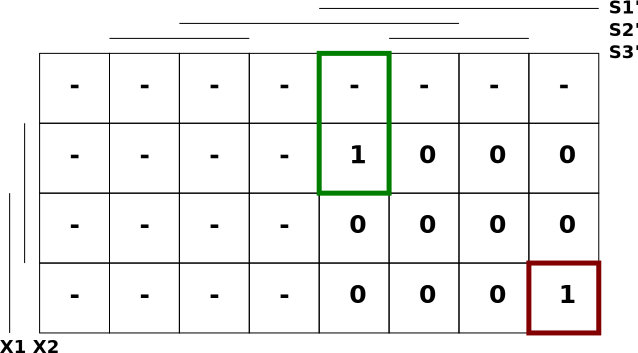
\includegraphics[width=\textwidth]{karnaugh_j1.pdf}
	\caption{$j_1$}
\end{minipage}
\begin{minipage}[b]{0.45\linewidth}
\includegraphics[width=\textwidth]{karnaugh_k1.pdf}
	\caption{$k_1$}
\end{minipage}
\end{figure}

\begin{figure}[ht!]
\begin{minipage}[b]{0.45\linewidth}
\includegraphics[width=\textwidth]{karnaugh_j2.pdf}
	\caption{$j_2$}
\end{minipage}
\begin{minipage}[b]{0.45\linewidth}
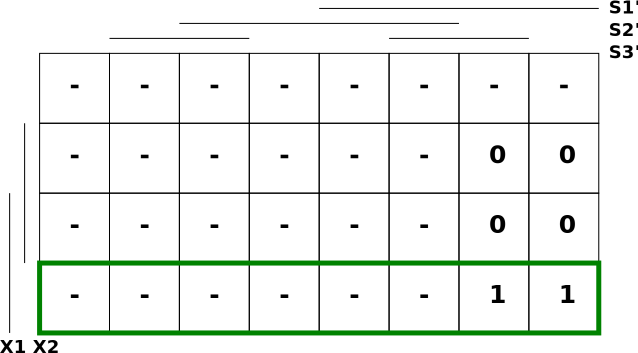
\includegraphics[width=\textwidth]{karnaugh_k2.pdf}
	\caption{$k_2$}
\end{minipage}
\end{figure}

\begin{figure}[ht!]
\begin{minipage}[b]{0.45\linewidth}
\includegraphics[width=\textwidth]{karnaugh_j3.pdf}
	\caption{$j_3$}
\end{minipage}
\begin{minipage}[b]{0.45\linewidth}
\includegraphics[width=\textwidth]{karnaugh_k3.pdf}
	\caption{$k_3$}
\end{minipage}
\end{figure}

\begin{figure}[ht!]
\begin{minipage}[b]{0.45\linewidth}
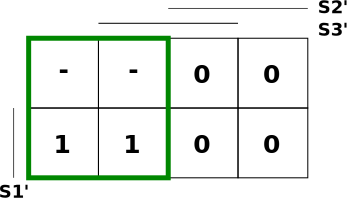
\includegraphics[width=\textwidth]{karnaugh_y1.pdf}
	\caption{$y_1$}
\end{minipage}
\begin{minipage}[b]{0.45\linewidth}
\includegraphics[width=\textwidth]{karnaugh_y2.pdf}
	\caption{$y_2$}
\end{minipage}
\end{figure}
\end{center}
\clearpage

\begin{align*}
j_1 &= x_1 \bar{s_1'} \bar{s_2'} s_3' + \bar{x_1} x_2 \bar{s_1'} s_2' s_3' \\
k_1 &= x_1 \\
j_2 &= \bar{x_1} x_2 \bar{s_1'} \bar{s_2'} s_3' \\
k_2 &= \bar{x_1} x_2 \\
j_3 &= x_1 s_1' + \bar{x_1} x_2 \bar{s_2'} \\
k_3 &= x_1 s_1' + \bar{x_1} x_2 \bar{s_1'} \\
y_1 &= s_2' \\
y_2 &= s_1' \bar{s_3'} + \bar{s_1'} \bar{s_2'} s_3 \\
\end{align*}

\clearpage
\begin{figure}[ht!]
\centering
	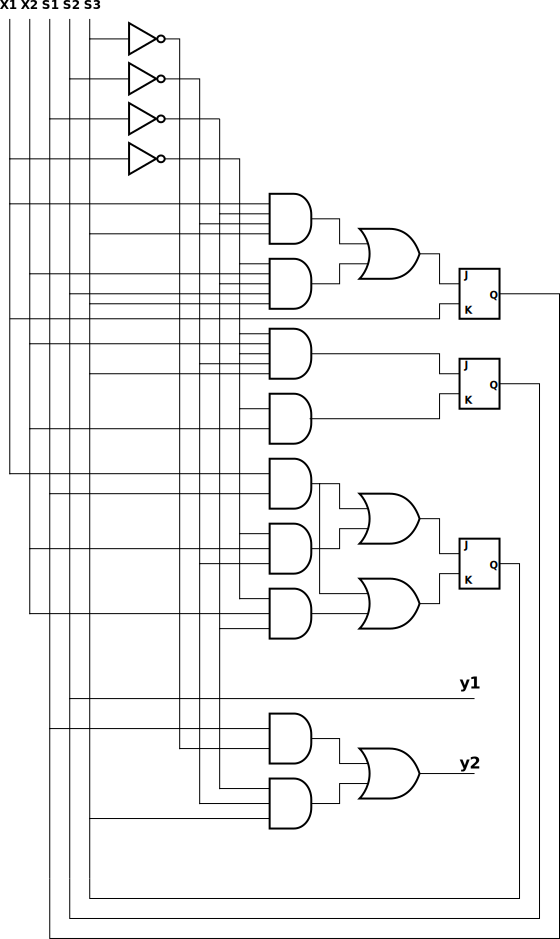
\includegraphics[height=.94\textheight]{obvod.pdf}
	\caption{Schéma sekvenčního obvodu}
\end{figure}

\end{document}
